% DO NOT COMPILE THIS FILE DIRECTLY!
% This is included by the other .tex files.

\begin{frame}[t,plain]
\titlepage
\end{frame}

\begin{frame}
\frametitle{MISP Galaxies}
    \begin{itemize}
    \item MISP started out as a platform for technical indicator sharing
    \item The need for a way to describe threat actors, tools and other commonalities became more and more pressing
    \item {\bf Taxonomies quickly became essential for classifying events}
    \item The weakness of the tagging aproach is that it's not very descriptive
    \item We needed a way to attach {\bf more complex structures to data}
    \item Also, with the different naming conventions for the same "thing" attribution was a mess
    \item This is where the Galaxy concept came in
    \end{itemize}
\end{frame}


\begin{frame}
\frametitle{Solution}
    \begin{itemize}
    	\item Pre-crafted galaxy "clusters" via GitHub project
        \item Attach them to an event and attribute(s)
    	\item The main design principle was that these higher level informations are meant for human consumption
    	\item This means flexibility - key value pairs, describe them dynamically
    	\item Technical indicators remain strongly typed and validated, galaxies are loose key value lists
    \end{itemize}
\end{frame}


\begin{frame}
\frametitle{The galaxy object stack}
    \begin{itemize}
    	\item {\bf Galaxy}: The type of data described (Threat actor, Tool, ...)
       	\item {\bf Cluster}: An individual instance of the galaxy (Sofacy, Turla, ...)
       	\item {\bf Element}: Key value pairs describing the cluster (Country: RU, Synonym: APT28, Fancy Bear)
       	\item {\bf Reference}: Referenced galaxy cluster (Such as a threat actor using a specific tool)
    \end{itemize}
\end{frame}

\begin{frame}
     \frametitle{(some) Existing galaxies}
     \begin{itemize}
        \item {\bf Exploit-Kit}: An enumeration of known exploitation kits used by adversaries
        \item {\bf Microsoft activity group}: Adversary groups as defined by Microsoft
        \item {\bf Preventive measure}: Potential preventive measures against threats
        \item {\bf Ransomware}: List of known ransomwares
        \item {\bf TDS}: Traffic Direction System used by adversaries
        \item {\bf Threat-Actor}: Known or estimated adversary groups
        \item {\bf Tool}: Tools used by adversaries (from Malware to common tools)
	\item {\bf MITRE ATT\&CK}: Adversarial Tactics, Techniques, and Common Knowledge (ATT\&CK™)
     \end{itemize}
\end{frame}

\begin{frame}
\frametitle{What a cluster looks like}
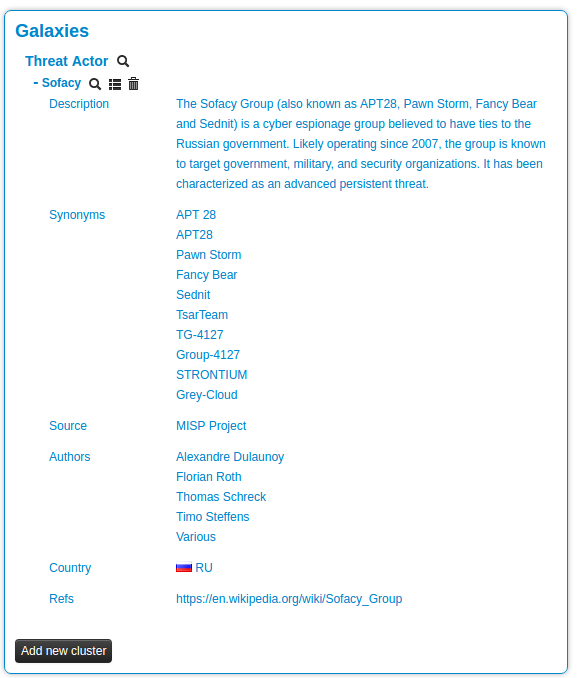
\includegraphics[scale=0.25]{screenshots/cluster.png}
\end{frame}

\begin{frame}
\frametitle{Attaching clusters to events}
    \begin{itemize}
    	\item Internally simply using a taxonomy-like tag to attach them to events
    	\item Example: misp-galaxy:threat-actor="Sofacy"
        \item {\bf Synchronisation works out of the box} with older instances too. They will simply see the tags until they upgrade.
       	\item Currently, as mentioned we rely on the community's contribution of galaxies
    \end{itemize}
\end{frame}

\begin{frame}
\frametitle{Attaching clusters}
	\begin{itemize}
		\item Use a searchable synonym database to find what you're after
	\end{itemize}
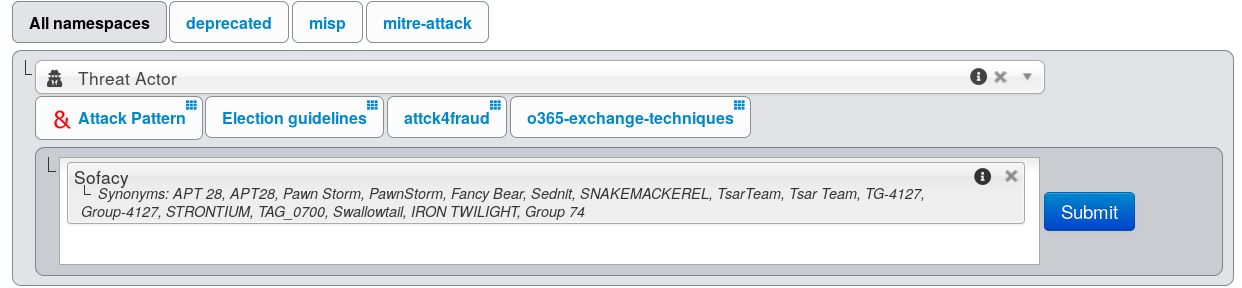
\includegraphics[scale=0.4]{screenshots/threatactor.png}
\end{frame}

\begin{frame}
\frametitle{Creating your own galaxy}
    \begin{itemize}
    	\item Creating galaxy clusters has to be straightforward to get the community to contribute
    	\item Building on the prior success of the taxonomies and warninglists
        \item Simple JSON format in similar fashion
        \item Just drop the JSON in the proper directory and let MISP ingest it
        \item We always look forward to contributions to our galaxies repository
    \end{itemize}
\end{frame}

\colorlet{punct}{red!60!black}
\definecolor{background}{HTML}{EEEEEE}
\definecolor{delim}{RGB}{20,105,176}
\colorlet{numb}{magenta!60!black}
\lstdefinelanguage{json}{
    basicstyle=\scriptsize,
    numbers=left,
    numberstyle=\scriptsize,
    stepnumber=1,
    numbersep=5pt,
    showstringspaces=false,
    breaklines=true,
    frame=lines,
    backgroundcolor=\color{background},
    literate=
     *{0}{{{\color{numb}0}}}{1}
      {1}{{{\color{numb}1}}}{1}
      {2}{{{\color{numb}2}}}{1}
      {3}{{{\color{numb}3}}}{1}
      {4}{{{\color{numb}4}}}{1}
      {5}{{{\color{numb}5}}}{1}
      {6}{{{\color{numb}6}}}{1}
      {7}{{{\color{numb}7}}}{1}
      {8}{{{\color{numb}8}}}{1}
      {9}{{{\color{numb}9}}}{1}
      {:}{{{\color{punct}{:}}}}{1}
      {,}{{{\color{punct}{,}}}}{1}
      {\{}{{{\color{delim}{\{}}}}{1}
      {\}}{{{\color{delim}{\}}}}}{1}
      {[}{{{\color{delim}{[}}}}{1}
      {]}{{{\color{delim}{]}}}}{1},
}


\begin{frame}[fragile]
	\frametitle{Galaxy JSON}
    \begin{itemize}
    	\item If you want to create a completely new galaxy instead of enriching an existing one
    \end{itemize}
    \begin{adjustbox}{keepaspectratio}
        \begin{lstlisting}[language=json,firstnumber=1]
{
   "name" : "Threat Actor",
   "type" : "threat-actor",
   "description": "Threat actors are characteristics of malicious actors (or adversaries) representing a cyber attack threat including presumed intent and historically observed behaviour.",
   "version": 1,
   "uuid": "698774c7-8022-42c4-917f-8d6e4f06ada3"
}
\end{lstlisting}
    \end{adjustbox}
\end{frame}

\begin{frame}[fragile]
	\frametitle{Cluster JSON}
    \begin{itemize}
    	\item Clusters contain the meat of the data
    	\item Skeleton structure as follows
    \end{itemize}
    \begin{adjustbox}{keepaspectratio}
        \begin{lstlisting}[language=json,firstnumber=1]
{
  "values": [
    {
      "meta": {},
      "description": "",
      "value": "",
      "related_clusters": [{}],
    }
  ]
}

\end{lstlisting}
    \end{adjustbox}
\end{frame}

\begin{frame}[fragile]
	\frametitle{Cluster JSON value example}
    \begin{adjustbox}{keepaspectratio}
        \begin{lstlisting}[language=json,firstnumber=1]
    {
      "meta": {
        "synonyms": [
            "APT 28", "APT28", "Pawn Storm", "Fancy Bear",
            "Sednit", "TsarTeam", "TG-4127", "Group-4127",
            "STRONTIUM", "Grey-Cloud"
        ],
        "country": "RU",
        "refs": [
          "https://en.wikipedia.org/wiki/Sofacy_Group"
        ]
      },
      "description": "The Sofacy Group (also known as APT28,
          Pawn Storm, Fancy Bear and Sednit) is a cyber
          espionage group believed to have ties to the
          Russian government. Likely operating since 2007,
          the group is known to target government, military,
          and security organizations. It has been
          characterized as an advanced persistent threat.",
      "value": "Sofacy"
    },

        \end{lstlisting}
    \end{adjustbox}
\end{frame}

\begin{frame}[fragile]
        \frametitle{meta best practices}
        \begin{itemize}
        \item Reusing existing values such as {\bf complexity, effectiveness, country, possible\_issues, colour, motive, impact, refs, synonyms, derivated\_from, status, date, encryption, extensions, ransomnotes, cfr-suspected-victims, cfr-suspected-state-sponsor, cfr-type-of-incident, cfr-target-category, kill\_chain}.
        \item Or adding your own meta fields.
        \end{itemize}
\end{frame}

\begin{frame}[fragile]
        \frametitle{meta best practices - a sample}
        \begin{adjustbox}{keepaspectratio}
          \begin{lstlisting}[language=json,firstnumber=1]
 {
      "description": "Putter Panda were the subject of an extensive report by CrowdStrike, which stated: 'The CrowdStrike Intelligence team has been tracking this particular unit since2012, under the codename PUTTER PANDA, and has documented activity dating back to 2007. The report identifies Chen Ping, aka cpyy, and the primary location of Unit 61486.'",
      "meta": {
        "cfr-suspected-state-sponsor": "China",
        "cfr-suspected-victims": [
          "U.S. satellite and aerospace sector"
        ],
        "cfr-target-category": [
          "Private sector",
          "Government"
        ],
        "cfr-type-of-incident": "Espionage",
        "country": "CN",
        "refs": [
          "http://cdn0.vox-cdn.com/assets/4589853/crowdstrike-intelligence-report-putter-panda.original.pdf",
          "https://www.cfr.org/interactive/cyber-operations/putter-panda"
        ],
        "synonyms": [
          "PLA Unit 61486",
          "APT 2",
          "Group 36",
          "APT-2",
          "MSUpdater",
          "4HCrew",
          "SULPHUR",
          "TG-6952"
        ]
      }}
          \end{lstlisting}
          \end{adjustbox}
\end{frame}

\begin{frame}[fragile]
        \frametitle{Galaxy JSON matrix-like}
        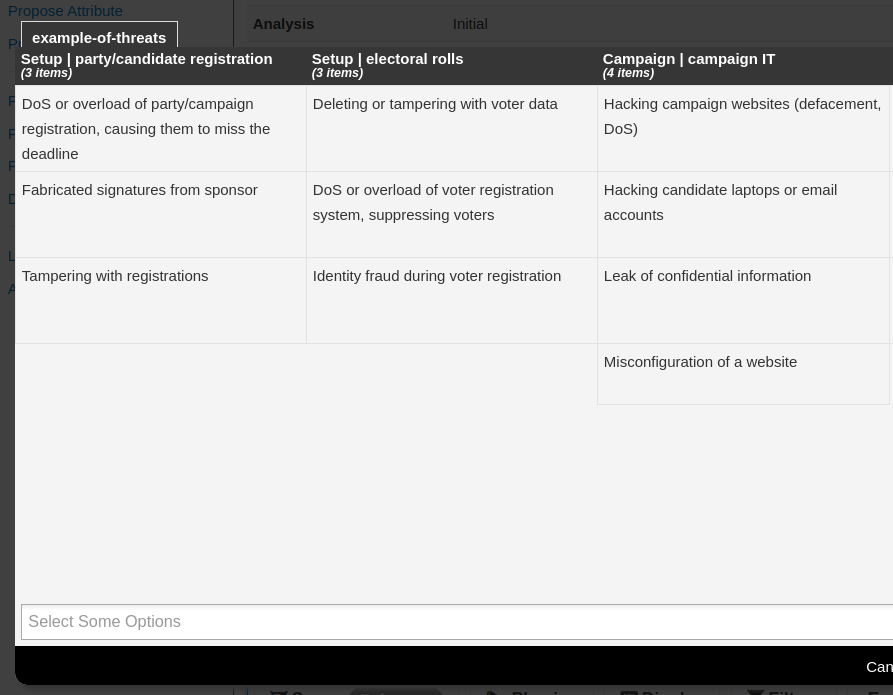
\includegraphics[width=0.9\linewidth]{screenshots/galaxy-matrix.png}
\end{frame}

\begin{frame}[fragile]
        \frametitle{Galaxy JSON matrix-like}
        \begin{adjustbox}{keepaspectratio}
            %\lstset{emph={kill_chain_order},emphstyle=\textbf}
            \begin{lstlisting}[language=json,firstnumber=1,escapechar=@]
        {
  "description": "Universal Development and Security Guidelines as Applicable to Election Technology.",
  "icon": "map",
  @\textbf{\color{red}"kill\_chain\_order": \{}@             @\textbf{\color{black}\textbackslash\textbackslash Tab in the matrix}@
      @\textbf{\color{red}"example-of-threats": [}@       @\textbf{\color{black}\textbackslash\textbackslash Column in the matrix}@
      @\textbf{\color{red}"setup | party/candidate-registration",}@
      @\textbf{\color{red}"setup | electoral-rolls",}@
      @\textbf{\color{red}"campaign | campaign-IT",}@
      @\textbf{\color{red}"all-phases | governement-IT",}@
      @\textbf{\color{red}"voting | election-technology",}@
      @\textbf{\color{red}"campaign/public-communication | media/press"}@
    @\textbf{\color{red}]}@
  @\textbf{\color{red}\},}@
  "name": "Election guidelines",
  "namespace": "misp",
  "type": "guidelines",
  "uuid": "c1dc03b2-89b3-42a5-9d41-782ef726435a",
  "version": 1
}
        \end{lstlisting}
        \end{adjustbox}
\end{frame}

\begin{frame}[fragile]
        \frametitle{Cluster JSON matrix-like}
        \begin{adjustbox}{keepaspectratio}
            \begin{lstlisting}[language=json,firstnumber=1, escapechar=@]
{
      "description": "DoS or overload of party/campaign registration, causing them to miss the deadline",
      "meta": {
        "date": "March 2018.",
         @\textbf{\color{red}"kill\_chain": [}@ @\textbf{\color{black}\textbackslash\textbackslash Define in which column the cluster should be placed}@
           @\textbf{\color{red}  "example-of-threats:setup | party/candidate-registration"}@
         @\textbf{\color{red}],}@
        "refs": [
          "https://www.ria.ee/sites/default/files/content-editors/kuberturve/cyber_security_of_election_technology.pdf"
        ]
      },
      "uuid": "154c6186-a007-4460-a029-ea23163448fe",
      "value": "DoS or overload of party/campaign registration, causing them to miss the deadline"
}
        \end{lstlisting}
        \end{adjustbox}
\end{frame}


\begin{frame}[fragile]
        \frametitle{Expressing relation between clusters}
        \begin{itemize}
                \item Cluster can be related to one or more clusters using default relationships from MISP objects and a list of tags to classify the relation.
        \end{itemize}

        \begin{lstlisting}[language=json,firstnumber=1]
        "related": [
        {
          "dest-uuid": "5ce5392a-3a6c-4e07-9df3-9b6a9159ac45",
          "tags": [
            "estimative-language:likelihood-probability=\"likely\""
          ],
          "type": "similar"
        }
      ],
      "uuid": "0ca45163-e223-4167-b1af-f088ed14a93d",
      "value": "Putter Panda"
        \end{lstlisting}
\end{frame}



\begin{frame}[fragile]
\frametitle{PyMISPGalaxies}
        \begin{adjustbox}{keepaspectratio}
\begin{lstlisting}[language=Python,basicstyle=\tiny]
from pymispgalaxies import Clusters
c = Clusters()
list(g.keys())
# ['threat-actor', 'ransomware', 'exploit-kit', 'tds', 'tool', 'rat', 'mitre-attack-pattern',
#  'mitre-tool', 'microsoft-activity-group', 'mitre-course-of-action', 'mitre-malware',
#  'mitre-intrusion-set', 'preventive-measure']
print(c.get("rat"))
# misp-galaxy:rat="Brat"
# misp-galaxy:rat="Loki RAT"
# misp-galaxy:rat="join.me"
# misp-galaxy:rat="Setro"
# misp-galaxy:rat="drat"
# misp-galaxy:rat="Plasma RAT"
# misp-galaxy:rat="NanoCore"
# misp-galaxy:rat="DarkTrack"
# misp-galaxy:rat="Theef"
# misp-galaxy:rat="Greame"
# misp-galaxy:rat="Nuclear RAT"
# misp-galaxy:rat="DameWare Mini Remote Control"
# misp-galaxy:rat="ProRat"
# misp-galaxy:rat="death"
# misp-galaxy:rat="Dark DDoSeR"
# ....
print(c.get("rat").description)
# remote administration tool or remote access tool (RAT), also called sometimes remote
# access trojan, is a piece of software or programming that allows a remote "operator"
# to control a system as if they have physical access to that system.
\end{lstlisting}
                \end{adjustbox}
\end{frame}


\begin{frame}
        \frametitle{Q\&A}
        \begin{itemize}
                \item info@circl.lu (if you want to join the CIRCL MISP sharing community)
                \item OpenPGP fingerprint: 3B12 DCC2 82FA 2931 2F5B 709A 09E2 CD49 44E6 CBCD
                \item \url{https://github.com/MISP/} - \url{http://www.misp-project.org/}
                \item We welcome any contributions to the project, be it pull requests, ideas, github issues,...
        \end{itemize}
\end{frame}

